\begin{frame}
  {Kernfragen in dieser Woche}
  \onslide<+->
  \onslide<+->
  \Large
  \centering 
  Wie kommt man von der Syntax zur Interpretation von Sätzen?\\
  \onslide<+->
  \Halbzeile
  Was \alert{bezeichnen} sprachliche Einheiten?\\
  \onslide<+->
  \Halbzeile
  Warum bezeichnen Sätze \alert{Wahrheitswerte}?\\
  \onslide<+->
  \Halbzeile
  Welche logischen Beziehungen bestehen zwischen Sätzen?\\
  \grau{Implikation vs.\ Präsupposition}\\
  \onslide<+->
  \Halbzeile
  Wie wird \alert{kleinschrittig natürlichsprachliche Semantik modelliert}?\\
  \onslide<+->
  \Halbzeile
  \grau{\footnotesize Das Wesentliche von heute in \citet[Kapitel~2]{ChierchiaMcconnellginet2000}}
\end{frame}

\section{Linguistische Theorien}

\begin{frame}
  {Ein neues semiotisches Dreieck}
  \onslide<+->
  \onslide<+->
  Im Sinn der letzten Woche interessiert uns nur die linke Seite.\\
  \onslide<+->
  \Zeile
  \centering 
  \begin{forest}
    [\gruen{Formen}
      [\gruen{Reale Objekte}, edge=gruen]
      [Mentale Konzepte]
    ]
  \end{forest}
\end{frame}

\begin{frame}
  {"`Semantik"' im generativen T-Modell}
  \onslide<+->
  \onslide<+->
  \centering 
  \resizebox{0.6\textwidth}{!}{
    \begin{tikzpicture}

      \node [rectangle, draw, align=left, color=teal, rounded corners=0.5em] (Numeration) at (5cm, -6cm) {Numeration};
      
      \node [visible on=<3->, rectangle, draw, align=left, color=gray] (Lexikon) at (1cm, -6cm) {Lexikon};
      \path (Lexikon.east) edge [visible on=<3->, line width=0.5mm, dashed] node [below, shift={(-0.4cm,0)}] {\textit{}} (Numeration.west);
     
      \node [visible on=<4->, rectangle, draw, align=left, color=gray] (Intention) at (9cm, -6cm) {Intention};
      \path (Intention.west) edge [visible on=<4->, line width=0.5mm, dashed] node [below, shift={(-0.4cm,0)}] {\textit{}} (Numeration.east);

      \node [visible on=<5->, rectangle, draw, align=left, fill=black, color=black, rounded corners=0.5em] (Syntax) at (5cm, -4.5cm) {\whyte{Syntax}};
      \path (Numeration.north) edge [visible on=<5->, line width=0.5mm, -latex] node [below, shift={(-0.4cm,0)}] {\textit{}} (Syntax.south);  

      \node [visible on=<6->, rectangle, draw, align=left, color=teal, rounded corners=0.5em] (Phrasenstruktur) at (5cm, -3cm) {Phrasenstruktur};
      \path (Syntax.north) edge [visible on=<6->, line width=0.5mm, -latex] node [below, shift={(-0.4cm,0)}] {\textit{}} (Phrasenstruktur.south);  

      \node [visible on=<7->, rectangle, draw, align=left, color=teal, rounded corners=0.5em] (PF) at (4cm, 0cm) {PF};
      \path (Phrasenstruktur.north) edge [visible on=<7->, line width=0.5mm, -latex] node [below, shift={(-0.4cm,0)}] {\textit{}} (PF.south);  
     
      \node [visible on=<8->, rectangle, draw, align=left, color=gray] (Aeusserung) at (1cm, 0cm) {Äußerung};
      \path (Aeusserung.east) edge [visible on=<8->, line width=0.5mm, dashed] node [below, shift={(-0.4cm,0)}] {\textit{}} (PF.west);
     
      \node [visible on=<9->, rectangle, draw, align=left, fill=black, color=black, rounded corners=0.5em] (Syntax2) at (6cm, -1.5cm) {\whyte{Syntax 2}};
      \path (Phrasenstruktur.north) edge [visible on=<9->, line width=0.5mm, -latex] node [below, shift={(-0.4cm,0)}] {\textit{}} (Syntax2.south);  
     
      \node [visible on=<10->, rectangle, draw, align=left, color=teal, rounded corners=0.5em] (LF) at (6cm, 0cm) {LF};
      \path (Syntax2.north) edge [visible on=<10->, line width=0.5mm, -latex] node [below, shift={(-0.4cm,0)}] {\textit{}} (LF.south);  

      \node [visible on=<11->, rectangle, draw, align=left, color=gray] (Interpretation) at (9cm, 0cm) {Interpretation};
      \path (Interpretation.west) edge [visible on=<11->, line width=0.5mm, dashed] node [below, shift={(-0.4cm,0)}] {\textit{}} (LF.east);
      
    \end{tikzpicture}
  }
\end{frame}

\begin{frame}
  {Repräsentationsebenen}
  \onslide<+->
  \onslide<+->
  Im klassischen generativen Modell:\\
  \grau{\footnotesize (In minimalistischen Modellen herrscht -- Chomsky muss es mögen! -- sowieso Anarchie.)}
  \Zeile
  \begin{itemize}[<+->]
    \item keine echte Interpretation auf LF
    \item Bewegung \rot{nachdem} der Satz geäußert wurde
    \item Herstellung einer logisch interpretierbaren \alert{Form} auf LF
    \item Grund | Syntax kann nicht alle Interpretationen abbilden
      \Halbzeile
      \begin{itemize}[<+->]
        \item[ ] \alert{Klassiker Quantorenskopus}
        \item[ ] \textit{Everybody loves somebody.}
          \Viertelzeile
        \item[A] Für alle Personen y gilt, dass es eine Person x gibt, für die gilt: y liebt x \grau{| $(\forall y)(\exists x)L(y,x)$}
        \item[B] Es gibt eine Person x, sodass für alle Personen y gilt: y liebt x \grau{| ($\exists x)(\forall y)L(y,x)$}
      \end{itemize}
  \end{itemize}
\end{frame}


\begin{frame}
  {Montagues direkte Interpretation}
  \onslide<+->
  \onslide<+->
  Sprache ist Logik ist Sprache \ldots\\
  \Halbzeile
  \begin{itemize}[<+->]
    \item[A] Entweder ist die \alert{Übersetzung in eine LF trivial und äquivalent zur PF\slash Syntax},\\
      oder \orongsch{sie fügt etwas hinzu, das der Sprache an sich fehlt}.
    \item[B] Sätze haben aber auch \alert{mit LF-Übersetzung nur die Bedeutungen,\\
      die sie sowieso haben} \grau{(keine Hinzufügung)}.
    \item[\ding{222}] Also ist die \gruen{Übersetzung in LF trivial und äquivalent zur PF\slash Syntax}.
    \item[\ding{222}] Wir können \gruen{Sätze direkt interpretieren} (wie sie gesprochen\slash geschrieben werden).
     \Zeile 
   \item \alert{Montagues \textit{lf}} | direkte Übersetzung von sprachlichen in logische Ausdrücke
  \end{itemize}
\end{frame}

\section{Referentielle Semantik basal}

\begin{frame}
  {Interessante Eigenschaften von Sprache}
  \onslide<+->
  \begin{itemize}[<+->]
    \item Aussagen über die\slash Teile der Welt
    \item Ausdrücke bezeichnen\slash referieren auf Dinge i.\,w.\,S.
    \item Informativität
    \item objektiv beurteilbar (\zB Wahrheit von Sätzen)
      \Zeile
    \item \alert{Aber welche sprachlichen Einheiten referieren auf was?}
  \end{itemize}
\end{frame}

\begin{frame}
  {Referenz | Eigennamen}
  \onslide<+->
  \onslide<+->
  Ein \alert{Eigenname} \ding{222} \alert{genau ein Objekt} in der Welt\\
  \onslide<+->
  \Zeile
  \centering
    \begin{tikzpicture}
      \node [] (name) at (-6cm, 0cm) {\textit{Jan Böhmermann}};
      \node [visible on=<4->] (boehmi) at (0cm, 0cm) {\includegraphics[width=0.2\textwidth]{\GRAPHPATH/boehmermann}};
      \path (name.east) edge [visible on=<4->, line width=0.5mm, -latex] node {\textit{}} (boehmi.west);
    \end{tikzpicture}
\end{frame}

\begin{frame}
  {Referenz | Appellativa}
  \onslide<+->
  \onslide<+->
  Ein normales \alert{Nomen} \ding{222} \alert{eine Menge von Objekten} in der Welt\\
  \onslide<+->
  \Zeile
  \centering
    \begin{tikzpicture}
      \node [] (noun) at (-6cm, 0cm) {\textit{soldier}};
      \node [visible on=<4->] (soldiers) at (0cm, 0cm) {
\includegraphics[width=0.2\textwidth]{\GRAPHPATH/soldiers}};
      \path (noun.east) edge [visible on=<4->, line width=0.5mm, -latex] node {\textit{}} (soldiers.west);
    \end{tikzpicture}
\end{frame}

\begin{frame}
  {Referenz | Adjektive und Verben}
  \onslide<+->
  \onslide<+->
  Ein (intersektives) \alert{Adjektiv} oder ein \alert{Verb} \ding{222} \alert{eine Menge von Objekten} in der Welt\\
  \onslide<+->
  \Zeile
  \centering
    \begin{tikzpicture}
      \node [] (adj) at (-6cm, 0cm) {\textit{human}};
      \node [visible on=<4->] (boehmi) at (0cm, +2cm) {\includegraphics[width=0.1\textwidth]{\GRAPHPATH/boehmermann}};
      \path (adj.east) edge [visible on=<4->, line width=0.5mm, -latex] node {\textit{}} (boehmi.west);
      \node [visible on=<5->] (soldiers) at (0cm, 0cm) {
\includegraphics[width=0.1\textwidth]{\GRAPHPATH/soldiers}};
      \path (adj.east) edge [visible on=<5->, line width=0.5mm, -latex] node {\textit{}} (soldiers.west);
      \node [visible on=<6->] (crowd) at (0cm, -2cm) {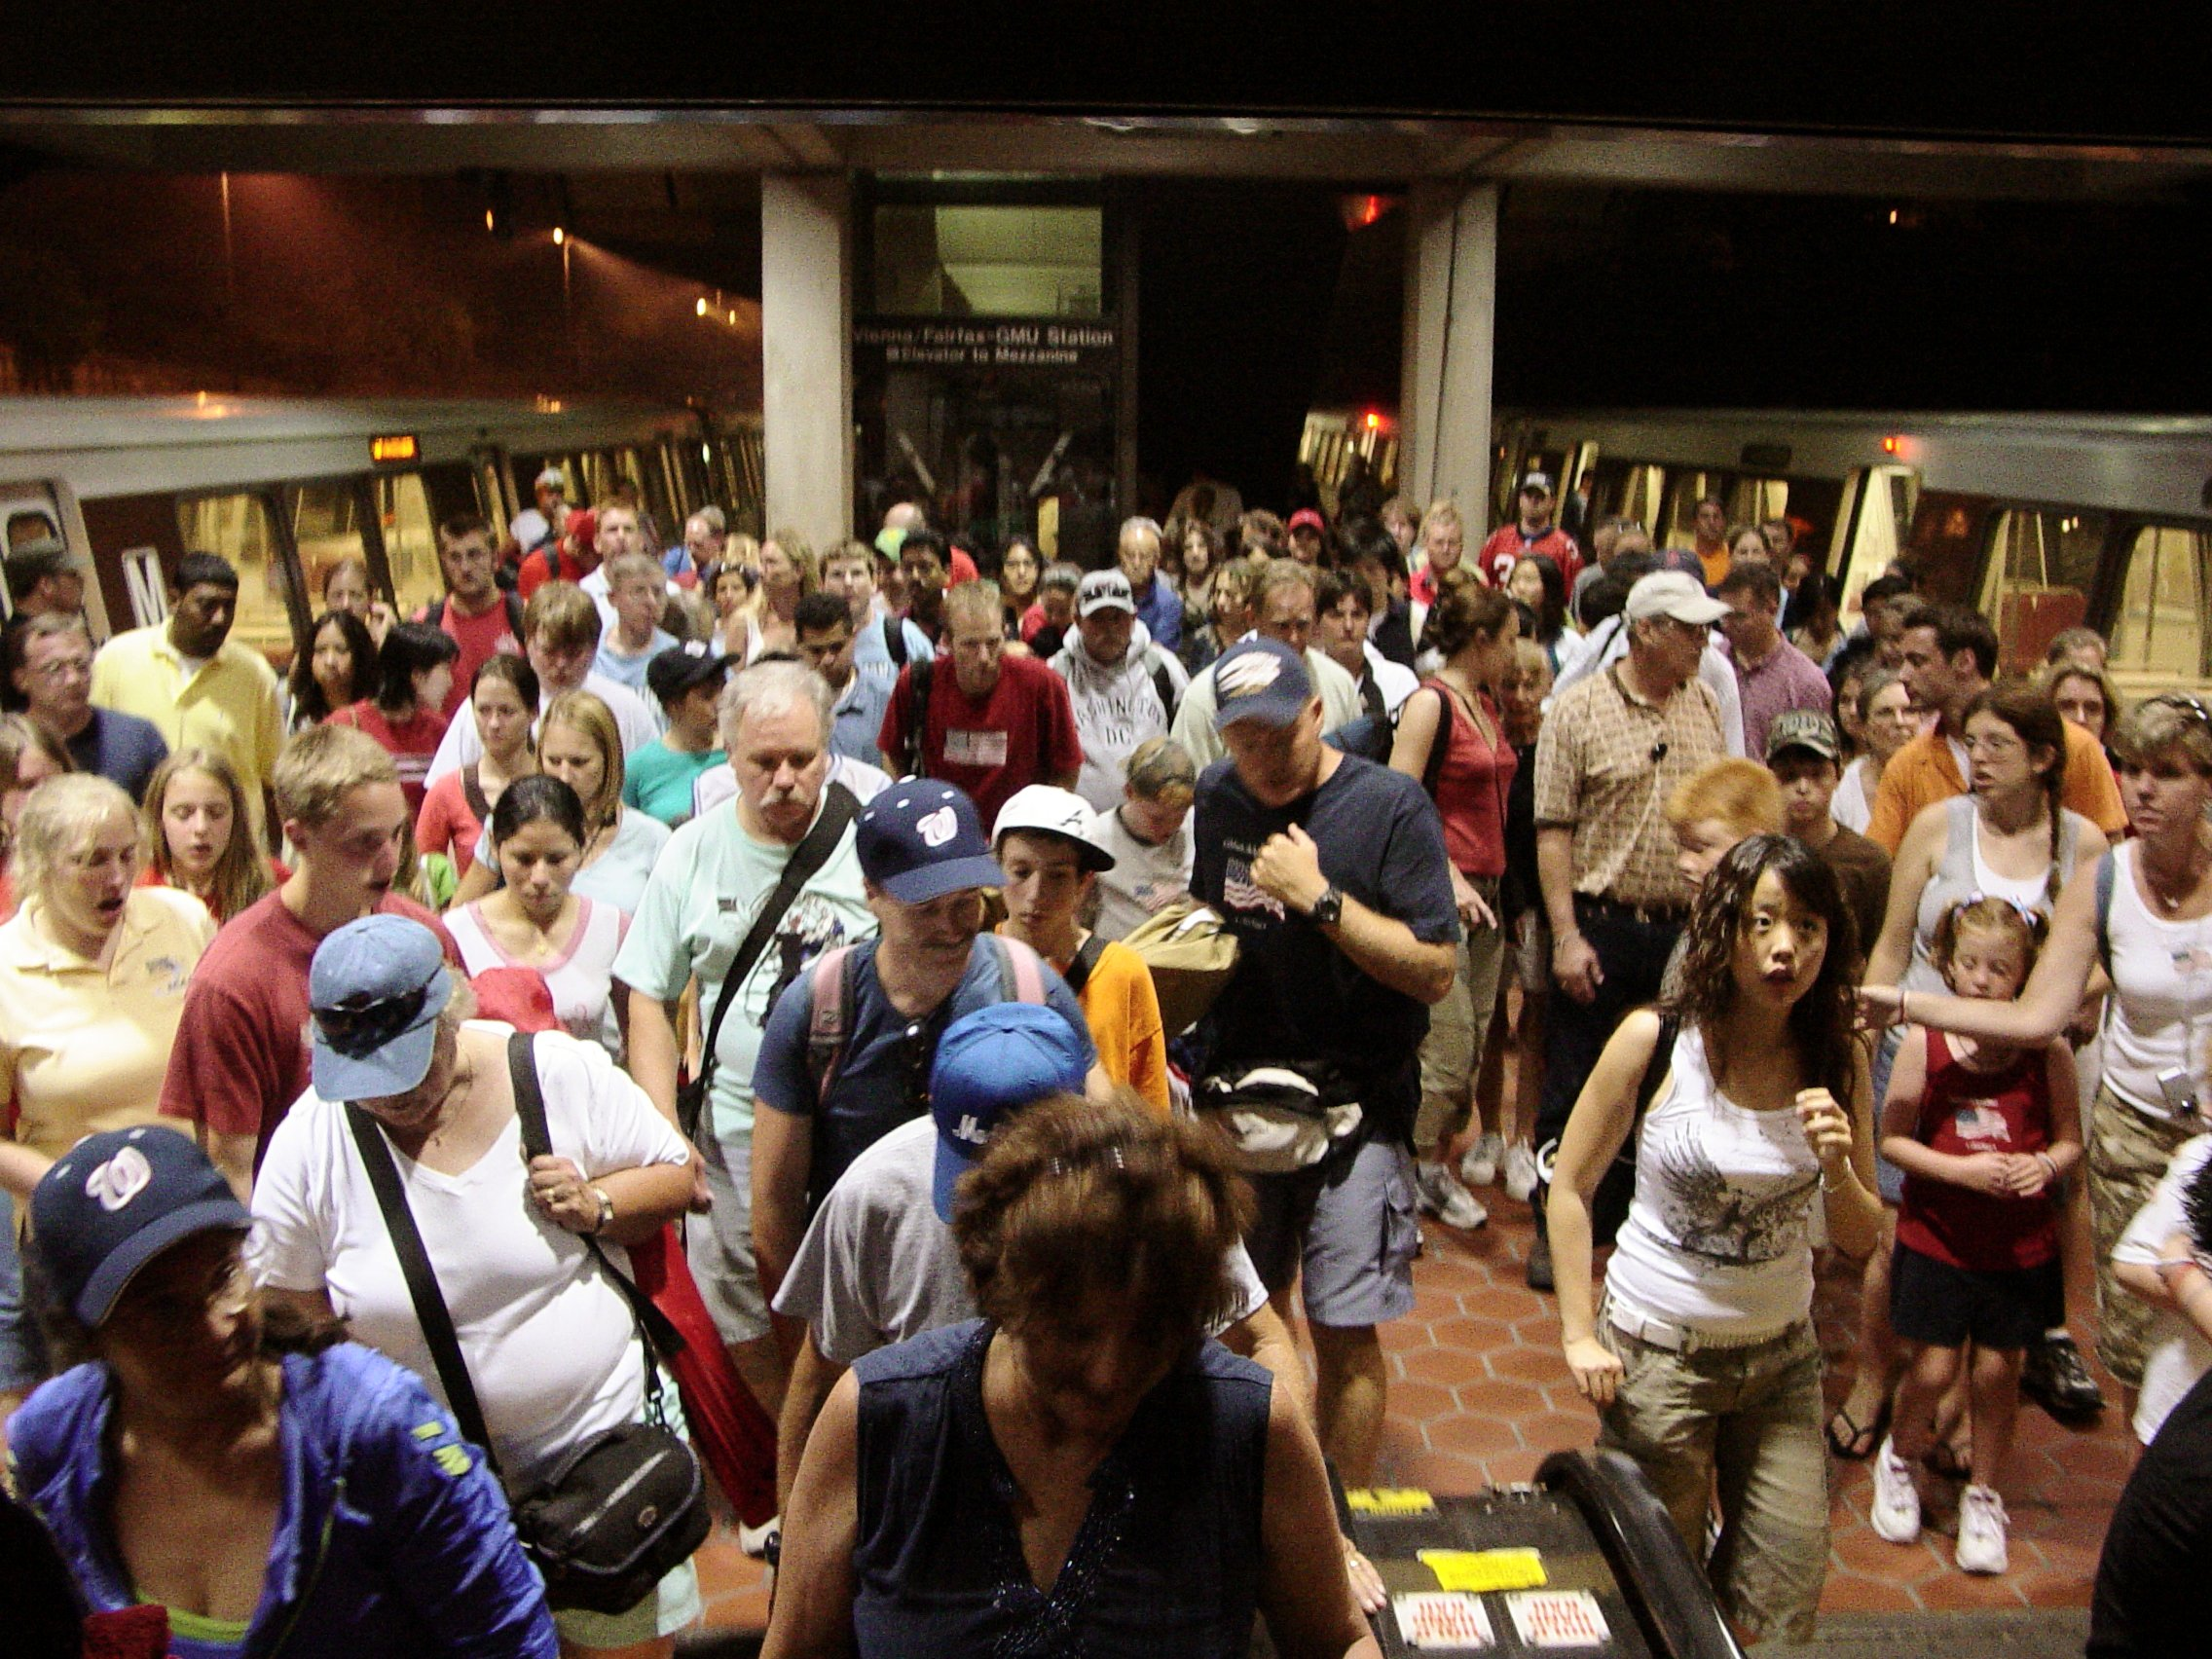
\includegraphics[width=0.1\textwidth]{\GRAPHPATH/crowd}};
      \path (adj.east) edge [visible on=<6->, line width=0.5mm, -latex] node {\textit{}} (crowd.west);
    \end{tikzpicture}
\end{frame}

\begin{frame}
  {Referenz | Sätze}
  \onslide<+->
  \onslide<+->
  Ein \alert{Satz} \ding{222} in erster Näherung \alert{ein Sachverhalt}\\
  \onslide<+->
  \Zeile
  \centering
    \begin{tikzpicture}
      \node [align=left] (s) at (-6cm, 0cm) {\it A humming bird\\\it is hovering over\\\it a red flower.};

      \node [visible on=<4->, align=center] (hum) at (0cm, +2cm) {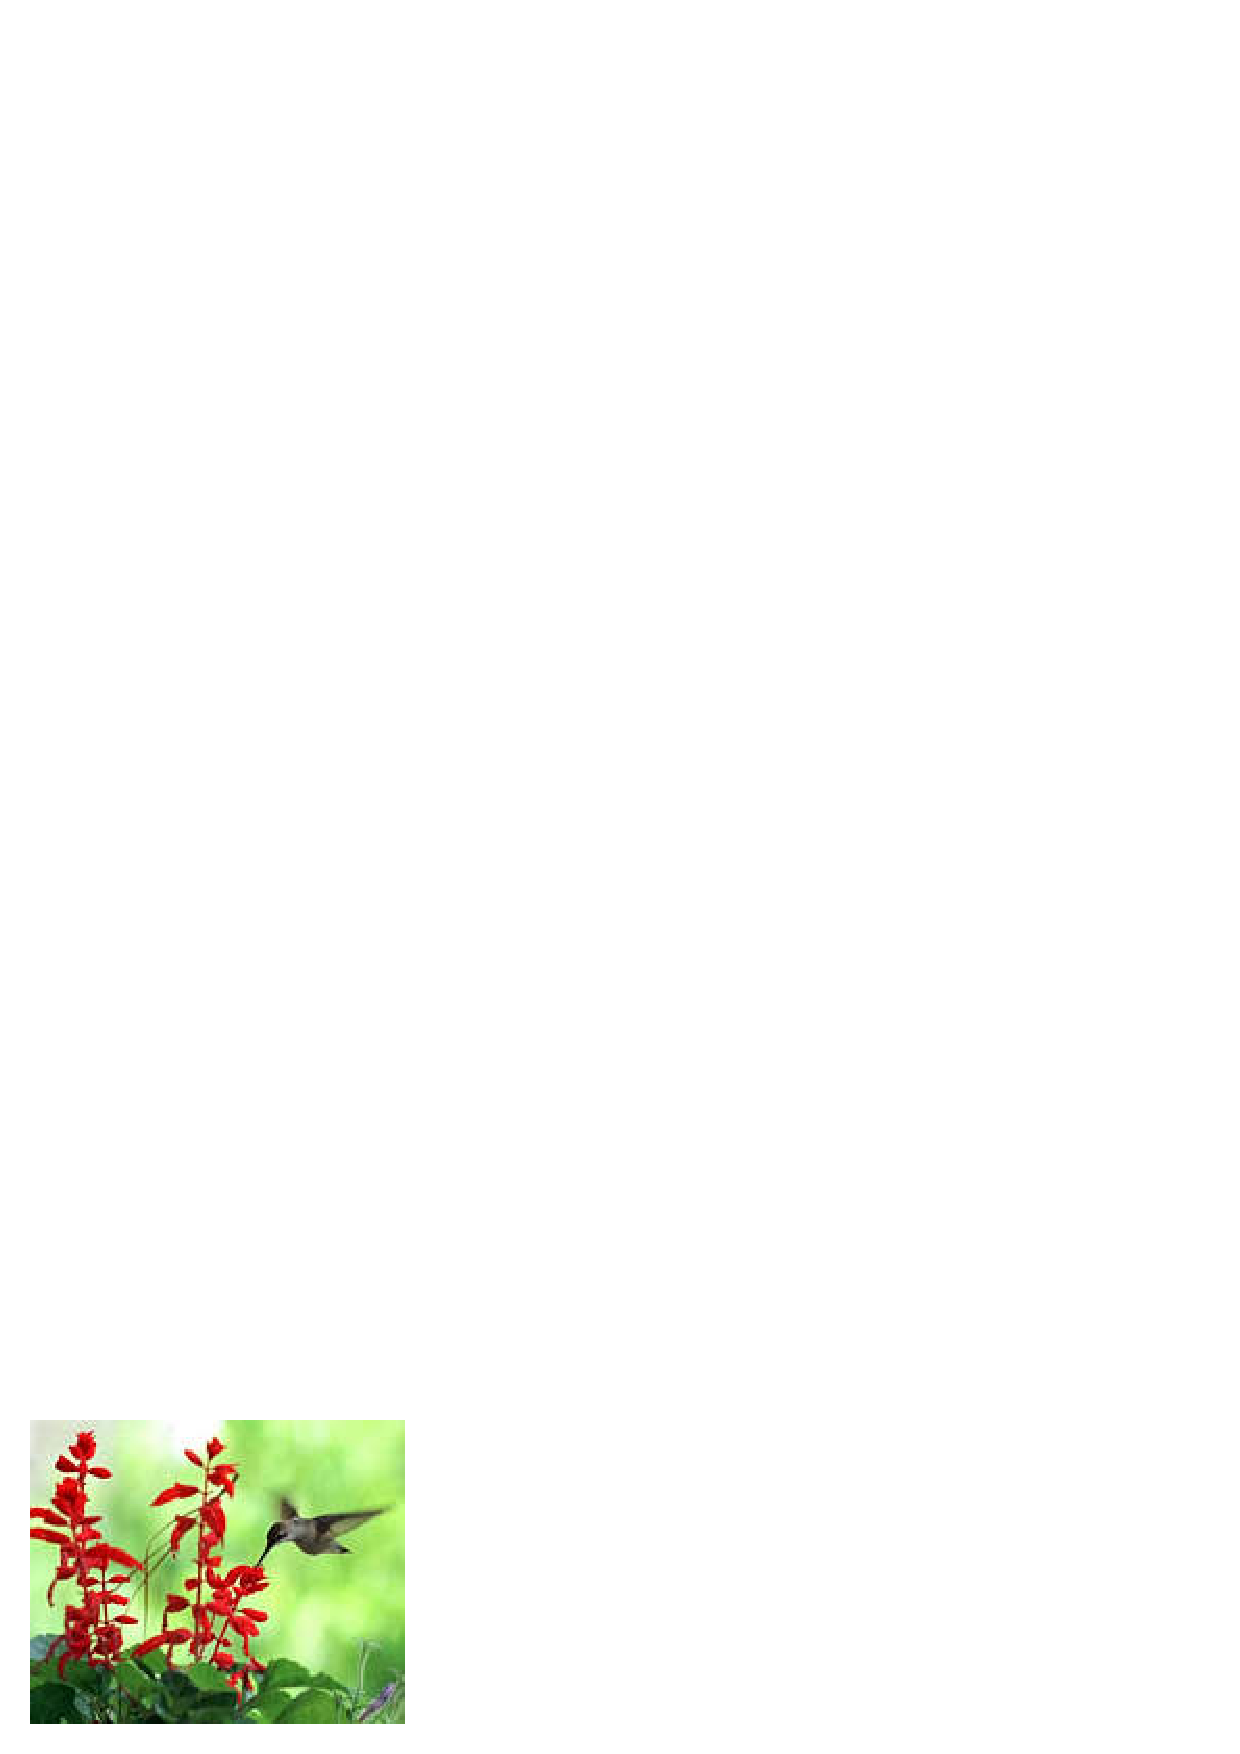
\includegraphics[width=0.2\textwidth]{\GRAPHPATH/hummingbird}};
      \path (s.east) edge [visible on=<4->, line width=0.5mm, -latex] node {\textit{}} (hum.west);
      
      \node [visible on=<5->, align=center] (boehmi) at (0cm, -2cm) {\includegraphics[width=0.2\textwidth]{\GRAPHPATH/boehmermann}\\\footnotesize (als Individuum)};
      \path (s.east) edge [visible on=<5->, line width=0.5mm, -latex, color=red] node {\textit{}} (boehmi.west);
      \node [visible on=<6->, align=center, color=red, fill=red] (nein) at (-3.5cm, -1.25cm) {\footnotesize \whyte{Nein! falsche}\\\footnotesize \whyte{Art von Objekt}};
    \end{tikzpicture}
\end{frame}

\begin{frame}
  {Freges Prinzip | Das hier wollen wir formalisieren!}
  \onslide<+->
  \onslide<+->
  Bedeutung ist kompositional!\\
  \Halbzeile
  \begin{itemize}[<+->]\small
    \item \textit{humming bird} \ding{222} die \alert{Menge} der Kolibri-Objekte
    \item \textit{a} \ding{222} \alert{Existenzaussage} für ein Element aus einer Menge
    \item \textit{a humming bird} \ding{222} \alert{Existenzaussage} für ein Element $x$\\
      aus der Menge der Kolibri-Objekte
    \item \textit{is hovering} \ding{222} die \alert{Menge} der schwebenden Objekten
    \item \textit{a humming bird is hovering} \ding{222} das existierende Kolibri-Objekt $x$\\
      ist auch ein \alert{Element der Menge} der schwebenden Objekte
    \item \textit{a red flower} \ding{222} \alert{Existenzaussage} für ein Element $y$\\
      aus der \alert{Schnittmenge} der roten Objekte und der Blumen-Objekte
    \item \textit{over} \ding{222} die \alert{Relation} zwischen Objekten (s.\ nächste Woche),\\
      die sich übereinander befinden
    \item \textit{A Humming is hovering over a red flower.} \ding{222}\\
      \gruen{Es gibt ein Objekt $x$ aus der Schnittmenge der Kolibri- und der schwebenden Objekte,\\
      und es gibt ein Objekt $y$ aus der Schnittmenge der roten und der Blumen-Objekte,\\
    und $x$ befindet sich über $y$.}
  \end{itemize}
\end{frame}

\section{Semantische Eigenschaften von Sätzen}

\begin{frame}
  {Implikation (Entailment)}
  \onslide<+->
  \onslide<+->
  Mengen von Aussagesätzen \alert{implizieren} andere Sätze.\\
  \onslide<+->
  Sätze (Implikationen) lassen sich aus anderen Sätzen (Axiome) \alert{beweisen}.\\
  \Halbzeile
  \begin{itemize}[<+->]
    \item[A] \textit{Jan Böhmermann ist ein Mensch.}
    \item[B] \textit{Jan Böhmermann ist leutselig.}
    \item[C] \textit{Jan Böhmermann ist ein leutseliger Mensch.}
      \Halbzeile
    \item[ ] \alert{$A,B\vdash C$} | A und B implizieren C. (C ist beweisbar aus A und B.)
    \item[ ] \rot{$A\not\vdash C$} | A impliziert nicht C.
    \item[ ] \rot{$B\not\vdash C$} | B impliziert nicht C.
      \Halbzeile
    \item[ ] \orongsch{$A\vdash A\wedge A$} \onslide<+->| \textit{Jan Böhmermann ist ein Mensch \orongsch{und} Jan Böhmermann ist ein Mensch.}
      \Halbzeile
    \item[D] \textit{Irgendetwas ist ein Mensch.}
    \item[ ] \alert{$A\vdash D$} 
  \end{itemize}
\end{frame}

\begin{frame}
  {Tests auf Implikation}
  \onslide<+->
  \onslide<+->
  Wenn diese Kriterien zutreffen, impliziert A B:\\
  \Zeile
  \begin{itemize}[<+->]
    \item Wenn A wahr ist, ist B auch immer wahr.
    \item Eine Situation, die von B beschrieben wird, wird auch von A beschrieben.
    \item Die Information in B ist vollständig in der Information in A enthalten.
    \item Man kann unter keinen Umständen sagen: \textit{A ist wahr, aber B ist nicht wahr.}
  \end{itemize}
\end{frame}

\begin{frame}
  {Übung | Sind das Implikationen?}
  \begin{itemize}[<+->]\small
    \item Böhmermann ist Showmaster. $\vdash$ Böhmermann ist menschlich.
    \item Böhmermann ist nicht sehr groß. $\vdash$ Irgendjemand ist nicht sehr groß.
    \item Böhmermann ist nicht sehr groß. $\vdash$ Irgendjemand ist sehr groß.
    \item Manche Menschen sind leutselig. $\vdash$ Böhmermann ist leutselig.
    \item Ich habe das neue drip-133-Album gehört. $\vdash$ drip-133 hat ein neues Album veröffentlicht.
    \item Nachdem ich einen Sherry getrunken habe, habe ich den Kondensator getauscht.\\
      $\vdash$ Ich habe einen Sherry getrunken.
    \item Nachdem Linux nicht mehr startete, habe ich einen weiteren Sherry getrunken.\\
      $\vdash$ Linux ist noch nie gestartet.
    \item Mein ehemaliger Mitbewohner mag Becks.\\
      $\vdash$ Mein ehemaliger Mitbewohner könnte Sherry mögen.
    \item Böhmermann hat das heutige ZDF Magazin beendet.\\
      $\vdash$ Das heutige ZDF Magazin wurde beendet.
  \end{itemize}
\end{frame}

\begin{frame}
  {Präsupposition | Der anzunehmende Hintergrund}
  \onslide<+->
  \onslide<+->
  Präsuppositionen sind schwächer als Implikationen.\\
  \Zeile
  \begin{itemize}[<+->]
    \item[A] \textit{Willy Brandt ist der gegenwärtige Kanzler Deutschlands.}
    \item[B] \textit{Wenn Willy Brandt der gegenwärtige Kanzler Deutschlands ist,\\
      trägt er eine große Verantwortung.}
    \item[C] \textit{Willy Brandt ist nicht der gegenwärtige Kanzler Deutschlands.}
    \item[D] \textit{Willy Brandt lebt.}
    \item[E] \textit{Es gibt einen Kanzler Deutschlands.}
      \Halbzeile
    \item \alert{A und B präsupponieren D.} = D ist eine Voraussetzung\\
      für eine erfolgreiche Interpretation von A und B.
    \item \orongsch{C präsupponiert nicht D.}
    \item \alert{A, B und C präsupponieren E.}
  \end{itemize}
\end{frame}

\begin{frame}
  {Tests auf Präsupposition}
  \onslide<+->
  \onslide<+->
  Die Unterschiede zur Implikation sind relevant.\\
  \Halbzeile
  \begin{itemize}[<+->]
    \item Nicht nur Aussagesätze haben Präsuppositionen (Modale, Konditionale, \ldots)
    \item Negierte Sätze haben oft gleiche Präsuppositionen wie nicht-negierte.
    \item Präsuppositionen können negiert werden, und der Ausgangssatz bleibt wahr.\\
      \grau{(Geht nicht mit Implikationen.)}
      \begin{itemize}[<+->]
        \item[F] \textit{Willy Brandt ist nicht der Kanzler Deutschlands.}
        \item[G] \textit{Es gibt einen Kanzler Deutschlands.}
        \item[ ] F präsupponiert G, bleibt aber wahr, wenn G falsch ist.
      \end{itemize}
  \end{itemize}
\end{frame}

\begin{frame}
  {Synonymie}
  \onslide<+->
  \onslide<+->
  Synonyme Ausdrücke haben \orongsch{exakt} \alert{die gleiche Referenz}.\\
  \Halbzeile
  \begin{itemize}[<+->]
    \item lexikalische Synonymie | \textit{humming bird} $\stackrel{lex}{\equiv}$ \textit{colibri}
      \Halbzeile
    \item kompositionale Synonymie
      \begin{itemize}[<+->]
        \item[ ] \textit{Mulder traf seine entführte Schwester, nachdem er\\
          in die geheime Militärbasis eingebrochen war.}
        \item[$\equiv$] \textit{Bevor er seine entführte Schwester traf,\\
          brach Mulder in die geheime Militärbasis ein.}
      \end{itemize}
    \Halbzeile
    \item \alert{$A\equiv B\ \text{gdw}\ A\vdash B\ \text{und}\ B\vdash A$} (gegenseitige Implikation)
    \item \grau{\textit{gdw} = \textit{genau dann wenn} | \textit{iff} = \textit{if and only if}}
  \end{itemize}
\end{frame}

\section{Referenz von Sätzen}

\begin{frame}
  {Natürliche Sprache und Implikation}
  \onslide<+->
  \onslide<+->
  Referentielle Semantik $\not=$ \alert{\textit{einfaches Zeigen auf Objekte durch Sprache}}.\\
  \Viertelzeile
  \onslide<+->
  Zusätzliche Logik für Fälle wie diesen (und viele andere):\\
  \Zeile
  \onslide<+->
  \begin{tabular}[h]{lll}
    & \alert{\textit{Die Lieblingsblume meines Kolibris}} & \textit{ist rot.} \\
    \visible<6->{\orongsch{$\vdash$}} & \visible<5->{\alert{\textit{Eine Blume}} & \textit{ist rot.}} \\
  \end{tabular}
\end{frame}

\begin{frame}
  {Sätze referieren aus Wahrheitswerte!}
  \onslide<+->
  \onslide<+->
  \centering 
  Um zu der gewünschten Logik zu kommen, zeigen wir jetzt,\\
  dass \alert{Sätze auf Wahrheitswerte referieren}.\\
  \Halbzeile
  \onslide<+->
  Wahrheitswerte sind nur \alert{\textit{wahr}} und \alert{\textit{falsch}}.\\
  \Halbzeile
  \onslide<+->
  Die Verben \alert{\textit{denotieren}} und \textit{\alert{referieren auf}} sind hier erst einmal synonym.\\
  \Doppelzeile
  \onslide<+->
  Warten Sie bitte ein paar Wochen, wenn Sie diese Darstellung reduktionistisch finden.
\end{frame}

\begin{frame}
  {Synonyme NPs}
  \onslide<+->
  \begin{itemize}[<+->]
    \item[a] \textit{colibri}
    \item[b] \textit{humming bird}
    \item[ ] \gruen{$a\stackrel{lex}{\equiv} b$}
      \Halbzeile
    \item[c] \textit{a brunette lady}
    \item[d] \textit{a brown-haired dame}
    \item[ ] \gruen{$c\equiv d$}
      \Halbzeile
    \item[e] \textit{the primates}
    \item[f] \textit{the apes and humans}
    \item[ ] \gruen{$e\equiv f$}
  \end{itemize}
\end{frame}

\begin{frame}
  {Synonymie von Konstituenten und Sätzen}
  Synonymie von Konstituenten im Satzkontext \ding{222} Satzsynonymie\\
  \onslide<+->
  \Halbzeile
  \begin{itemize}[<+->]
    \item[A] \alert{\textit{A \orongsch{colibri} is hovering over a red flower.}}
    \item[B] \alert{\textit{A \orongsch{humming bird} is hovering over a red flower.}}
    \item[ ] \gruen{$A\equiv B$ weil $a\equiv b$ und Satzkontext identisch}
    \item[ ] \gruen{$[\Sub{A} a]\equiv[\Sub{B} b]$ wenn $a\equiv b$ und $[\Sub{A} \_]=[\Sub{B} \_]$}
      \Halbzeile
    \item[C] \alert{\textit{Lauren Bacall was \orongsch{a brunette lady}.}}
    \item[D] \alert{\textit{Lauren Bacall was \orongsch{a brown-haired dame}.}}
    \item[ ] \gruen{$C\equiv D$ weil $c\equiv d$ und Satzkontext identisch}
      \Halbzeile
    \item[E] \alert{\textit{\orongsch{Primates} are intelligent.}}
    \item[F] \alert{\textit{\orongsch{The apes and humans} are intelligent.}}
    \item[ ] \gruen{$E\equiv F$ weil $e\equiv f$ und Satzkontext identisch}
  \end{itemize}
\end{frame}

\begin{frame}
  {Zwei Axiome}
  \onslide<+->
  \begin{itemize}[<+->]
    \item[ ] Referenz\slash Denotat eines Ausdrucks A als \alert{\den{A}}\\
      \grau{$\dem{\cdot}$ ist eine Funktion!}
      \Zeile
    \item[ ] Erinnerung: Synonymität von Sätzen ist gegenseitige Implikation.
      \Zeile
    \item[Ax1] Synonyme Ausdrücke (NPs, Verben, Sätze, \ldots) haben dieselbe Referenz.
    \item[ ] Formal: \alert{$A\equiv B\leftrightarrow\den{A}=\den{B}$}
      \Zeile
    \item[Ax2] Wenn wir in Ausdruck C einen Ausdruck A durch\\
      einen synonymen Ausdruck B ersetzen, behält C seine Referenz.
    \item[ ] Formal: \alert{$\den{A}=\den{B}\rightarrow\den{[\Sub{C} A]}=\den{[\Sub{C} B]}$}
  \end{itemize}
\end{frame}

\begin{frame}
  {Zwei wahre Sätze}
  \onslide<+->
  \onslide<+->
  Wahrheitswert von A und B | \alert{1} bzw.\ \alert{\textit{wahr}} bzw.\ \alert{\textit{true}} oder \alert{\textit{T}}\\
  \Zeile
  \begin{itemize}[<+->]
    \item[A] \textit{Lauren Bacall was a brunette lady.}
    \item[B] \textit{My humming bird's favourite flower is red.} 
  \end{itemize}
  \Doppelzeile
  \centering \alert{\Large Diese Sätze haben außer ihrem Wahrheitswert\\
  semantisch nichts gemein!}
\end{frame}

\begin{frame}
  {Erste Schlussfolgerung}
  \onslide<+->
  \onslide<+->
  Einsetzen von A und B in \alert{Satzkontext T bzw. $[\Sub{T}\_]$} (Aussage über Wahrheitswert)\\
  \Halbzeile
  \begin{itemize}[<+->]
    \item[T] \alert{\textit{The truth value of `\_' is 1.}}
      \Halbzeile
    \item[{[\Sub{T}A]}] \alert{\textit{The truth value of `\orongsch{Lauren Bacall was a brunette lady.}' is 1.}}
    \item[{[\Sub{T}B]}] \alert{\textit{The truth value of `\orongsch{My humming bird's favourite flower is red.}' is 1.}}
      \Halbzeile
    \item[ ] Da aus $A$ $[_T A]$ folgt und umgekehrt: \gruen{$A\equiv[\Sub{T}A]$} und \gruen{$B\equiv[\Sub{T}B]$}
    \item[ ] und daher mit Ax1 \gruen{$\den{A}=\den{[\Sub{T}A]}$} und \gruen{$\den{B}=\den{[\Sub{T}B]}$}
      \Halbzeile
    \item[ ] Bitte bedenken: $A$ und $[\Sub{T}A]$ haben auch intuitiv "`denselben Inhalt"'.
  \end{itemize}
\end{frame}

\begin{frame}
  {Zweite Schlussfolgerung}
  \onslide<+->
  \onslide<+->
  In $[\Sub{T}A]$ und $[\Sub{T}B]$ sind A und B jeweils in einer NP eingebettet.\\
  \Halbzeile
  \begin{itemize}[<+->]
    \item $\den{the truth value of A}=\den{the truth value of B}=1$
    \item[ ] mit Ax2 \gruen{$\den{[\Sub{T}A]}=\den{[\Sub{T}B]}$}
    \item[ ] damit \gruen{$\den{A}=\den{[\Sub{T}A]}=\den{[\Sub{T}B]}=\den{B}=1$}
      \Halbzeile
    \item \gruen{Sätze referieren auf Wahrheitswerte.}\\
      \grau{(Denn man kann das mit zwei beliebigen wahren Sätzen machen.)}
    \item Achtung | \gruen{Wahrheitswerte sind auch nur realweltliche Objekte.}
  \end{itemize}
\end{frame}

\begin{frame}
  {Adäquatheit von Wahrheitswerten als Satzreferenten}
  \onslide<+->
  \onslide<+->
  Nicht so \rot{sinnlos}, \rot{schwachsinnig}, \rot{inhaltsleer}, \ldots\ wie oft vermutet\\
  \Zeile
  \begin{itemize}[<+->]
    \item Referentielle Semantik
      \begin{itemize}[<+->]
        \item Analyse der Referenten verschiedener Typen von Ausdrücken
        \item Komposition von Sätzen
        \item deduktive Logik für Sätze
        \item \alert{Benennen der Wahrheitsbedingungen} (\ding{222} Modelltheorie)
      \end{itemize}
      \Halbzeile
    \item minimale Gemeinsamkeit \alert{aller} Sätze
    \item gut formal berechenbar (Binarität)
    \item reichhaltigere Semantik später (basierend auf Wahrheitswerten)
  \end{itemize}
\end{frame}

\section{Reden in Fragmenten}

\begin{frame}
  {Grammatik- und Semantikfragmente}
  \onslide<+->
  \onslide<+->
  \alert{Konstruktive}, \alert{schrittweise} Annäherungen an sprachliche Modellierung\\
  \Zeile
  \begin{itemize}[<+->]
    \item Grammatikfragment | Ausschnitt einer Gesamtgrammatik
    \item erwünschte schrittweise Erweiterung von Fragmenten (vgl.\ HPSG)
      \Zeile
    \item Konstruktion eines Semantik-Fragments
      \begin{itemize}[<+->]
         \item grammatische Kategorien und Referenzen von Wörtern
         \item Grammatikmechanismen und zugehörige Bedeutungskonstruktion
         \item Ergebnis | Semantik von Sätzen und Beitrag aller Konstituenten dazu
      \end{itemize}
    \item \Halbzeile
      \alert{T-Sätze}
      \begin{itemize}[<+->]
        \item \alert{L} eine Sprache, \alert{S} ein Satz, \alert{v} ein Sachverhalt, \alert{p} eine Aussage über Wahrheitsbedingungen
        \item \alert{S aus L ist wahr in v gdw p.}
      \end{itemize}
  \end{itemize}
\end{frame}

\begin{frame}
  {Das Lexikon}
  \onslide<+->
  \onslide<+->
  Die folgenden simplexen Ausdrücke sind Teil von F\Sub{1}.\\
  \onslide<+->
  Kein anderer simplexer Ausdruck ist Teil von F\Sub{1}.\\
  \Halbzeile
  \begin{enumerate}[<+->]
    \item N $\rightarrow$ \emph{Herr Webelhuth, Frau Klenk, the Turm-Mensa} \label{lex01}
    \item V\Sub{{i}} $\rightarrow$ \emph{is relaxed, is creative, is stupid} \label{lex02}
    \item V\Sub{t} $\rightarrow$ \emph{prefers} \label{lex03}
    \item conj $\rightarrow$ \emph{and, or} \label{lex04}
    \item neg $\rightarrow$ \emph{it is not the case that} \label{lex05}
  \end{enumerate}
\end{frame}

\begin{frame}
  {Die Phrasenstrukturgrammatik von F\Sub{1}}
  \onslide<+->
  \onslide<+->
  Folgende Kompositionsregeln sind Teil von F\Sub{1}.\\
  Keine andere Kompositionsregel ist Teil von F\Sub{1}.\\
  \Halbzeile
  \begin{enumerate}[<+->]
    \item S $\rightarrow$ N VP \label{syn01}
    \item S $\rightarrow$ S conj S \label{syn02}
    \item S $\rightarrow$ neg S \label{syn03}
    \item VP $\rightarrow$ V\Sub{{i}} \label{syn04}
    \item VP $\rightarrow$ V\Sub{t} N \label{syn05}
  \end{enumerate}
\end{frame}

\begin{frame}
  {Referenz simplexer Ausdrücke}
  \begin{itemize}[<+->]
    \item $\llbracket$Herr Webelhuth$\rrbracket$ = Herr Webelhuth \label{lexint01}
    \item $\llbracket$Frau Klenk$\rrbracket$ = Frau Klenk \label{lexint02}
    \item $\llbracket$the Turm-Mensa$\rrbracket$ = the Turm-Mensa \label{lexint03}
    \item $\llbracket$is relaxed$\rrbracket$ = $\{x:x\ is\ relaxed\}$ \label{lexint04}
    \item $\llbracket$is creative$\rrbracket$ = $\{x:x\ is\ creative\}$ \label{lexint05}
    \item $\llbracket$is stupid$\rrbracket$ = $\{x:x\ is\ stupid\}$ \label{lexint06}
    \item $\llbracket$prefers$\rrbracket$ = $\{\langle x,y\rangle: x\ prefers\ y\}$ \label{lexint07}
  \end{itemize}
\end{frame}

\begin{frame}
  {Referenz von Funktionswörtern}
  Funktionswörter referieren auf \alert{Funktionen}.\\
  \Zeile
  \begin{itemize}[<+->]
    \item $\dem{neg} = \left[
                       \begin{array}{l}
                                1 \rightarrow 0\\
                                0 \rightarrow 1
                       \end{array}
                     \right]$ \label{fint01}
    \item $\dem{and} = \left[
                       \begin{array}{l}
                                \langle 1,1 \rangle \rightarrow 1\\
                                \langle 1,0 \rangle \rightarrow 0\\
                                \langle 0,1 \rangle \rightarrow 0\\
                                \langle 0,0 \rangle \rightarrow 0
                       \end{array}
                       \right]$ \label{fint02}
    \item $\dem{or} = \left[
                           \begin{array}{l}
                                    \langle 1,1 \rangle \rightarrow 1\\
                                    \langle 1,0 \rangle \rightarrow 1\\
                                    \langle 0,1 \rangle \rightarrow 1\\
                                    \langle 0,0 \rangle \rightarrow 0
                           \end{array}
                           \right]$ \label{fint03}
  \end{itemize}
\end{frame}

\begin{frame}
  {T-Sätze für F\Sub{1}}
  \begin{itemize}[<+->]
    \item \den{\alert{[\Sub{S}{ }N{ }VP]}} = 1 iff $\den{N}\in\den{VP}$, else $0$ \label{t01}
    \item \den{\alert{[\Sub{S} S1 conj S2]}} = $\den{conj}(\langle\den{S1},\den{S2}\rangle)$ \label{t02}
    \item \den{\alert{[\Sub{S} neg S]}} = $\den{neg}(\den{S})$ \label{t03}
    \item \den{\alert{[\Sub{VP} V\Sub{t} N]}} = $\{x:\langle x,\den{N}\rangle\in\den{V\Sub{t}}\}$ \label{t04}
      \Halbzeile
    \item für einen nicht verzweigenden Knoten K und seine Tochter D: $\dem{[\Sub{K} D]}=\dem{D}$ \label{t05}
      \Halbzeile
    \item \grau{Das geht alles eleganter. Bitte etwas Geduld!}
  \end{itemize}
\end{frame}

\begin{frame}
  {Schritt 1 | Syntax parsen}
  Ist folgendes ein Satz aus F\Sub{1}? \onslide<+-> \alert{\textit{Herr Webelhuth is relaxed.}}\\
  \Halbzeile
  \begin{itemize}[<+->]
    \item{} [\Sub{N} \textit{Herr Webelhuth}] mit \gruen{Lexikonregel \ref{lex01}}
    \item{} [\Sub{V\Sub{i}} \textit{is relaxed}] mit \gruen{Lexikonregel \ref{lex02}}
    \item{} [\Sub{VP} [\Sub{V\Sub{i}} \textit{is relaxed}]] mit \gruen{Syntaxregel \ref{syn04}}
    \item{} [\Sub{S} [\Sub{N} \textit{Herr Webelhuth}] \Sub{VP} [\Sub{V\Sub{i}} \textit{is relaxed}]] mit \gruen{Syntax \ref{syn01}}
  \end{itemize}
\end{frame}

\begin{frame}
  {Syntax als Baum}
  \centering 
  \begin{forest}
    [S
      [N
        [\textit{Herr Webelhuth}]
      ]
      [VP
        [V\Sub{i}
          [\textit{is relaxed}]
        ]
      ]
    ]
  \end{forest}
\end{frame}

\begin{frame}
  {Semantik | Referenz der Teile und ihrer Bedeutung}
  \onslide<+->
  \onslide<+->
  \alert{v} (Sachverhalt) | Herr Webelhuth (das ontologische Objekt) $\in\{x: x\ is\ relaxed\}$\\
  \Halbzeile
  \begin{itemize}[<+->]
    \item für N: \den{\textit{Herr Webelhuth}} = Herr Webelhuth (das ontologische Objekt)
    \item für VP (und V\Sub{i}): \den{\textit{is relaxed}} = $\{x:x\ is\ relaxed\}$ (enthält Herrn Webelhuth)
    \item für S: \den{[\Sub{S}{ }N{ }VP]} = 1 iff \den{N} $\in$ \den{VP}, else 0
      \Halbzeile
    \item in v daher \gruen{\den{[\Sub{S} \textit{Herr Webelhuth is relaxed.}]}=1}
  \end{itemize}
\end{frame}

\begin{frame}
  {Semantik als Baum}
  \begin{tabular}[h]{cc}
  \onslide<+->
  \onslide<+->
  \centering 
  \begin{forest}
    [\den{S}
      [\den{N}
        [\den{\textit{Herr Webelhuth}}]
      ]
      [\den{VP}
        [\den{V\Sub{i}}
          [\den{\textit{is relaxed}}]
        ]
      ]
    ]
  \end{forest} &%
  \begin{forest}
    [\gruen{1} \alert{because Herr Webelhuth$\in$\{x:x is relaxed\}}
      [\grau{Herr Webelhuth}
        [\gruen{Herr Webelhuth}]
      ]
      [\grau{\{x:x is relaxed\}}
        [\grau{\{x:x is relaxed\}}
          [\gruen{\{x:x is relaxed\}}]
        ]
      ]
    ]
  \end{forest}
  \\
  \end{tabular}
\end{frame}

\begin{frame}
  {Komplexere Phrasenstrukturen}
  \alert{[\Sub{S\Sub{1}} \textit{Frau Klenk is creative}]} \textit{and it is not the case that} \orongsch{[\Sub{S\Sub{2}} \textit{Herr Webelhuth is relaxed}]}\\
  and \gruen{[\Sub{S\Sub{3}} \textit{Frau Klenk prefers the Turm-Mensa}]}.\\
  \Halbzeile
  \centering
  \centering
  \scalebox{0.8}{
    \begin{forest}
      [S
        [\alert{S\Sub{1}}, bluetree
          [N, bluetree
            [\textit{Frau Klenk}]
          ]
          [VP, bluetree
            [\textit{is creative}, narroof]
          ]
        ]
        [conj
          [\textit{and}]
        ]
        [S
          [neg
            [\textit{it is not the case that}]
          ]
          [S
            [S\Sub{2}, orongschtree
              [N, orongschtree
                [\textit{Herr Webelhuth}]
              ]
              [VP, orongschtree
                [\textit{is relaxed}, narroof]
              ]
            ]
            [conj]
            [S\Sub{3}, gruentree
              [N, gruentree
                [\textit{Frau Klenk}]
              ]
              [VP, gruentree
                [V\Sub{t}, gruentree
                  [\textit{prefers}]
                ]
                [N, gruentree
                  [\textit{the Turm-Mensa}]
                ]
              ]
            ]
          ]
        ]
      ]
    \end{forest}
  }
\end{frame}

\begin{frame}
  {Interpretation}
  \onslide<+->
  \onslide<+->
  Die Situation\slash die Umstände v sind:\\
  \Halbzeile
  \begin{itemize}[<+->]
    \item $\text{Herr Webelhuth}\in\{x: x\text{ is relaxed}\}$
    \item $\text{Frau Klenk}\in\{x: x\text{ is creative}\}$
    \item $\langle\text{Frau Klenk, Turm-Mensa}\rangle\not\in\{\langle x,y\rangle: x\text{ prefers }y\}$
  \end{itemize}
\end{frame}


\begin{frame}
  {Die Interpretation komplexerer Phrasenstrukturen \only<30>{ist einfach!}}
  \onslide<+->
  \onslide<+->
  \begin{itemize}
    \item \orongsch<13->{$\text{Herr Webelhuth}\in\{x: x\text{ is relaxed}\}$}
    \item \alert<8->{$\text{Frau Klenk}\in\{x: x\text{ is creative}\}$}
    \item \gruen<21->{$\langle\text{Frau Klenk, Turm-Mensa}\rangle\not\in\{\langle x,y\rangle: x\text{ prefers }y\}$}
  \end{itemize}
  \onslide<+->
  \Halbzeile
  \centering
  \scalebox{0.55}{
    \begin{forest}
      [\alt<1-29>{\den{S}}{1}
        [\alt<1-7>{\den{\alert{S\Sub{1}}}}{1}, bluetree
          [\alt<1-4>{\den{N}}{Frau Klenk}, bluetree
            [\alt<1-3>{\den{\textit{Frau Klenk}}}{Frau Klenk}]
          ]
          [\alt<1-6>{\den{VP}}{\{x: x is creative\}}, bluetree
            [\alt<1-5>{\den{\textit{is creative}}}{\{x: x is creative\}}, narroof]
          ]
        ]
        [\alt<1-28>{\den{conj}}{
                \scalebox{0.6}{$\left[
                       \begin{array}{l}
                                \langle 1,1 \rangle \rightarrow 1\\
                                \langle 1,0 \rangle \rightarrow 0\\
                                \langle 0,1 \rangle \rightarrow 0\\
                                \langle 0,0 \rangle \rightarrow 0
                       \end{array}
                     \right]$}
        }
          [\alt<1-27>{\den{\textit{and}}}{
                \scalebox{0.6}{$\left[
                       \begin{array}{l}
                                \langle 1,1 \rangle \rightarrow 1\\
                                \langle 1,0 \rangle \rightarrow 0\\
                                \langle 0,1 \rangle \rightarrow 0\\
                                \langle 0,0 \rangle \rightarrow 0
                       \end{array}
                     \right]$}
          }]
        ]
        [\alt<1-26>{\den{S}}{1}
          [\alt<1-25>{\den{neg}}{
              \scalebox{0.6}{$\left[
                       \begin{array}{l}
                                1 \rightarrow 0\\
                                0 \rightarrow 1
                       \end{array}
                     \right]$}
          }
            [\alt<1-24>{\den{\textit{it is not the case that}}}{
              \scalebox{0.6}{$\left[
                       \begin{array}{l}
                                1 \rightarrow 0\\
                                0 \rightarrow 1
                       \end{array}
                     \right]$}
            }]
          ]
          [\alt<1-23>{\den{S}}{0}
            [\alt<1-12>{\den{S\Sub{2}}}{1}, orongschtree
              [\alt<1-9>{\den{N}}{Herr Webelhuth}, orongschtree
                [\alt<1-8>{\den{\textit{Herr Webelhuth}}}{Herr Webelhuth}]
              ]
              [\alt<1-11>{\den{VP}}{\{x: x is relaxed\}}, orongschtree
                [\alt<1-10>{\den{\textit{is relaxed}}}{\{x: x is relaxed\}}, narroof]
              ]
            ]
            [\alt<1-22>{\den{conj}}{
                \scalebox{0.6}{$\left[
                       \begin{array}{l}
                                \langle 1,1 \rangle \rightarrow 1\\
                                \langle 1,0 \rangle \rightarrow 0\\
                                \langle 0,1 \rangle \rightarrow 0\\
                                \langle 0,0 \rangle \rightarrow 0
                       \end{array}
                     \right]$}
            }
              [\alt<1-21>{\den{\textit{and}}}{
                \scalebox{0.6}{$\left[
                       \begin{array}{l}
                                \langle 1,1 \rangle \rightarrow 1\\
                                \langle 1,0 \rangle \rightarrow 0\\
                                \langle 0,1 \rangle \rightarrow 0\\
                                \langle 0,0 \rangle \rightarrow 0
                       \end{array}
                     \right]$}
              }]
            ]
            [\alt<1-20>{\den{S\Sub{3}}}{0}, gruentree
              [\alt<1-14>{\den{N}}{Frau Klenk}, gruentree
                [\alt<1-13>{\den{\textit{Frau Klenk}}}{Frau Klenk}]
              ]
              [\alt<1-19>{\den{VP}}{\{$\langle$x,the Turm-Mensa$\rangle$: x prefers the Turm-Mensa\}}, gruentree
                [\alt<1-18>{\den{V\Sub{t}}}{\{$\langle$x,y$\rangle$: x prefers y\}}, gruentree
                  [\alt<1-17>{\den{\textit{prefers}}}{\{$\langle$x,y$\rangle$: x prefers y\}}]
                ]
                [\alt<1-16>{\den{N}}{the Turm-Mensa}, gruentree
                  [\alt<1-15>{\den{\textit{the Turm-Mensa}}}{the Turm-Mensa}]
                ]
              ]
            ]
          ]
        ]
      ]
    \end{forest}
  }
\end{frame}

\begin{frame}
  {Das war aber nicht alles}
  \onslide<+->
  \onslide<+->
  Der zuletzt analysierte Satz ist \alert{strukturell ambig}, und\\
  und mit der strukturellen geht eine \alert{semantische Ambiguität} einher.\\
  \onslide<+->
  \Zeile
  \centering 
  \orongsch{Hausaufgabe: Analysieren Sie die Syntax und Semantik des Satzes\\
    in der anderen Lesart nur mit den Mitteln von F\Sub{1}.}
\end{frame}


\begin{frame}
  {Zusatzaufgabe}
  \onslide<+->
  \onslide<+->
  \small Entwickeln Sie ein ähnliches Fragment D\Sub{1} für das Deutsche mit Lexikon, Syntax und Semantik\\
  das die folgenden Sätze generiert. Lexikon und Konstituentenstruktur können Sie frei wählen.\\
  \Halbzeile
  \grau{\scriptsize Es hat einen guten Grund, dass wir oft Englisch als Objektsprache nehmen. Sie können für dieses\\
  Fragment des Deutschen Kasus entweder ignorieren, oder Sie probieren, Kasusunterschiede zu modellieren.}\\
  \onslide<+->
  \Halbzeile
  \begin{itemize}[<+->]
    \item Herr Müller ist Aktivist.
    \item Frau Klann ist intelligent.
    \item Frau Klann begrüßt Herrn Müller.
    \item Frau Klann hustet.
    \item Frau Klann schreibt ein gutes Buch.
  \end{itemize}
\end{frame}
